% Tipo de documento y paquetes a utilizar.
\documentclass[12pt]{article}
\usepackage[utf8]{inputenc}
% \usepackage{amsmath, amsthm, amsfonts, mathtools} % Paquete para usar más fórmulas y ecuaciones.
\usepackage{graphicx}       % Paquete para usar imágenes y figuras.
\usepackage{geometry}       % Paquete para trabajar con los márgenes del documento.
\usepackage{fancyhdr}       % Paquete para personalizar encabezado y pie de página.
\usepackage{lastpage}       % Paquete para referenciar páginas del documento.
\usepackage{listings}       % Paquete para escribir código de programación.
\usepackage{inconsolata}    % Paquete de tipo de letra consola.
\usepackage{multirow}       % Paquete para combinar filas y columnas en tablas.
\usepackage{array}          % Paquete para trabajar tablas especializadas.
\usepackage{xcolor}         % Paquete básico para agregar color al texto.
\usepackage{float}          % Paquete para utilizar fijación de figuras H.
\usepackage{hyperref}       % Paquete para insertar links en el documento.

% Define colores nuevos.
\definecolor{color}{HTML}{E4E4EE}
\definecolor{verde}{HTML}{3C8031}

% Personalización de la fuente para el código.
\lstset{
    language = HTML,                    % Lenguaje con palabras reservadas de este resaltadas.
    basicstyle = \ttfamily\footnotesize,% Utiliza la fuente tttfamily, en especial el paquete inconsolata.
    frame = single,                     % Quita el marco al cuadro flotante que contiene el código o texto.
    backgroundcolor = \color{color},    % Cambia el color del fondo del marco del código. Utiliza el paquete "xcolor" y define un nuevo color.
    columns = fullflexible,             % Ajusta el cuadro flotante al tamaño del texto del documento.
    breaklines = true,                  % Ajusta el texto dentro del contenedor.
    inputencoding = utf8,               % Admite caracteres del código UTF8.
    extendedchars = true,               % Soporte para caracteres especiales.
    %numbers = left,                    % Agrega número de línea al código (izquierda, sin número y derecha).
    showstringspaces = false,           % Quita los guiones bajos predeterminados de los espacios en cadenas de texto.
    escapebegin = \obeyspaces,          % Complemento de la entrada anterior.
    % rulecolor = \color{red},          % Color del borde del marco del código.
    % numberstyle = \color{red},        % Color de los números en el texto o código.
    % stringstyle = \color{red},        % Color de las cadenas de texto en el texto o código.
    % keywordstyle = \color{red},       % Color de las palabras reservadas en el texto o código.
    % identifierstyle = \color{red},    % Color del texto o código.
    commentstyle = \color{verde},       % Color de los comentarios en el texto o código.
    literate =                          % Acepta los siguientes caracteres especiales fuera de UTF8.
        {á}{{\'a}}1 {é}{{\'e}}1 {í}{{\'i}}1 {ó}{{\'o}}1 {ú}{{\'u}}1
        {Á}{{\'A}}1 {É}{{\'E}}1 {Í}{{\'I}}1 {Ó}{{\'O}}1 {Ú}{{\'U}}1
        {ñ}{{\~n}}1 {Ñ}{{\~N}}1,
}

% Márgenes del documento.
\newgeometry{
    top=2.5cm,     % Superior.
    bottom=2.5cm,  % Inferior.
    outer=2.5cm,   % Parte exterior.
    inner=2.5cm,    % Parte interior.
}

% Personalización de la cabecera y pie de página.
\pagestyle{fancy}
\fancyhf{}
\rhead{Overleaf}                                            % Texto en esquina superior derecha.
\lhead{Apuntes de HTML}                                     % Texto en esquina superior izquierda.
\rfoot{Pagina \thepage \hspace{1pt} de \pageref{LastPage}}  % Texto en esquina inferior derecha (Página n de n).
% Ancho de línea horizontal superior e inferior.
\renewcommand{\headrulewidth}{1pt}
\renewcommand{\footrulewidth}{1pt}

% Datos para la portada del documento.
\title{Apuntes de HTML}
\author{migueluisV}
\date{Realizadas: Diciembre 2022}

% Inicio del documento.
\begin{document}

% Cambia los títulos de los índices:
% Content - Índice
% List of Figures - Índice de Figuras
% List of Tables - Índice de Tablas
\renewcommand*\contentsname{Índice}
\renewcommand{\listtablename}{Índice de Tablas}
\renewcommand{\listfigurename}{Índice de Figuras}

% Inserta la portada y los índices.
\maketitle\newpage
\tableofcontents\newpage
\listoffigures\newpage
\listoftables\newpage

\hspace{0.55cm}Este documento se hizo con \href{https://es.overleaf.com/}{\textbf{Overleaf}} y los ejemplos fueron desarrollados y probados con \textbf{Visual Studio Code}, con su extensión \textbf{Live Server} en el buscador \textbf{Microsoft Edge} o \textbf{Brave}, por lo que algunas propiedades puede que lleguen a requerir un \textit{Prefijo de buscador} para funcionar.

\sloppy La estructura HTML de los ejemplos en este documento serán omitidos, dejando únicamente lo vital para que los ejemplos funcionen y para evitar que este trabajo sea muy largo, en caso de que sea necesario la estructura completa, se incluirá.

% Incluye los archivos que conforman al proyecto.
\section{HTML básico}
\hspace{0.55cm}Las etiquetas que siempre debe contener un documento \textit{.html} o \textit{.htm} son:
\begin{lstlisting}
    <html>
        <head>
        </head>
        <body>
            This is a line of text.
        </body>
    </html>
\end{lstlisting}


\subsection{Tipos de etiquetas}
\begin{itemize}
    \item \textbf{Block-levels}: establecen una estructura o característica primordial dentro de la estructura HTML, suelen ser la cabecera o contenedor de otras etiquetas, y dan un salto de línea cuando estas etiquetas se cierran.
    \item \textbf{Inline}: son aquellas etiquetas que no van dentro de otras para dar formato al contenido de las mismas, y no dan un salto de línea cuando se cierran.
    \item Existen elementos que son Block-level e Inline, algunos ejemplos son:
    \begin{itemize}
        \item \textbf{applet}: subprograma Java embebido.
        \item \textbf{iframe}: estructura frame.
        \item \textbf{ins}: texto insertado.
        \item \textbf{map}: mapa de imagen.
        \item \textbf{object}: objetos embebidos.
        \item \textbf{scritp}: un script dentro del documento HTML.
    \end{itemize}
    \item Los elementos Inline no pueden contener elementos Block-level.
\end{itemize}


\subsection{Etiquetas básicas de HTML}
\begin{itemize}
    \item \textbf{p}: agrega un párrafo de texto al sitio o página.
    \item \textbf{span}: contiene texto en el sitio o página.
    \item \textbf{h, h1 h2, ..., h6}: agrega un título 1, título 2, ..., hasta título 6 al sitio o página. No es recomendable utilizar los títulos solamente para hacer grande el texto, ya que los buscadores los utilizan para indexar el sitio o página con la web.
    \item \textbf{title}: es el título de la pestaña del sitio o página.
    \item \textbf{hr/}: crea una línea horizontal. \textbf{No requiere de una etiqueta de comienzo.}
    \item \textbf{br/}: agrega un espacio en blanco o salto de línea. \textbf{No requiere de una etiqueta de comienzo}.
    \item \textbf{div}: es un elemento Block-level que suele ser utilizado para contener otras etiquetas.
\end{itemize}

Un ejemplo del aspecto de las etiquetas anteriormente mencionadas es el siguiente código y la \textit{Figura \ref{fig: 1}}:
\begin{lstlisting}
    <!-- Tipos de encabezados. -->
    <h1>Título 1</h1>
    <h2>Título 1.1</h2>
    <h3>Título 1.1.1</h3>
    <h4>Título 1.1.1.1</h4>
    <h5>Título 1.1.1.1.1</h5>
    <h6>Título 1.1.1.1.1.1</h6>

    <!-- Etiquetas para objetos. -->
    <p>Esto es un párrafo, contenido en un P,<br/>acabo de dar un salto de línea con BR.</p>
    <span>Esto es otro párrafo, contenido en un SPAN.</span>
    
    <!-- Salto de línea. -->
    <hr/>
    
    <!-- Contenedor que almacena un párrafo. -->
    <div>
        <p>Esto es otro párrafo, separado de los demás con una línea horizontal HR; contenido en un P dentro de un contenedor DIV.</p>
    </div>
\end{lstlisting}
\begin{figure}[H]
    \centering
    \caption{Vista de las etiquetas básicas}
    \label{fig: 1}
    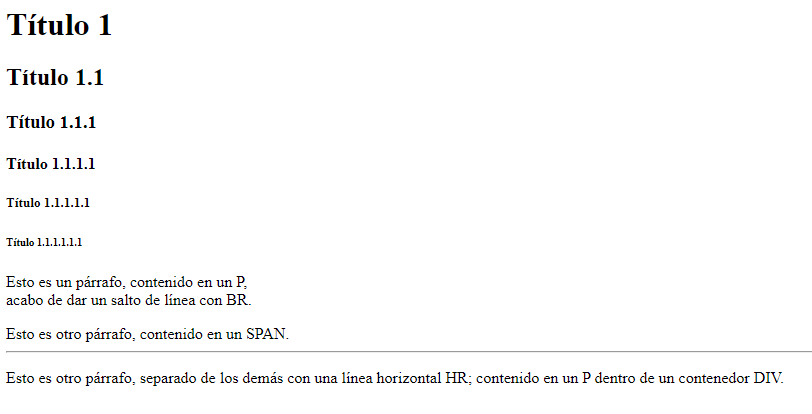
\includegraphics[width=12cm]{ss_html/etiquetas_basicas.png}
\end{figure}


\subsection{Etiquetas de formato}
\begin{itemize}
    \item \textbf{b}: vuelve el texto negrita.
    \item \textbf{big}: vuelve un texto un poco más grande.
    \item \textbf{i}: vuelve el texto cursiva.
    \item \textbf{small}: vuelve el texto un poco más pequeño.
    \item \textbf{strong}: resalta un texto importante con negritas.
    \item \textbf{em}: resalta un texto importante con cursiva.
    \item \textbf{sub}: posiciona un texto en un subíndice.
    \item \textbf{sup}: posiciona un texto en un superíndice.
    \item \textbf{ins}: subraya un texto.
    \item \textbf{del}: tacha un texto.
\end{itemize}

Un ejemplo del aspecto de las etiquetas anteriormente mencionadas es el siguiente código y la \textit{Figura \ref{fig: 2}}:
\begin{lstlisting}
    <b>Este texto es negrita.</b><br/>
    
    <strong>Este texto es negrita e importante para el buscador.</strong><br/>
    
    <i>Este texto es cursiva.</i><br/>
    
    <em>Este texto es cursiva e importante para el buscador.</em><br/>
    
    <ins>Este texto está subrayado.</ins><br/>
    
    <del>Este texto está tachado</del><br/>
    
    <big>Este texto es más grande.</big><br/>
    
    <small>Este texto es más pequeño.</small><br/>
    
    <sup>Este texto tiene un <sup>super índice.</sup><br/>
    
    <sub>Este texto tiene un <sub>sub índice.</sub>
\end{lstlisting}
\begin{figure}[H]
    \centering
    \caption{Vista de las etiquetas de formato}
    \label{fig: 2}
    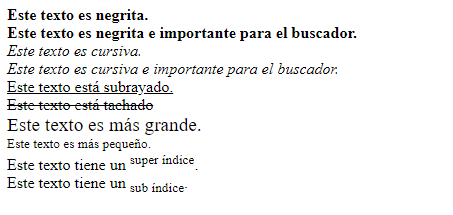
\includegraphics[width=11cm]{ss_html/etiquetas_formato.png}
\end{figure}


\subsection{Atributos de etiquetas}
\hspace{0.55cm}Son información adicional que modifican a la etiqueta. Estos atributos poseen valores.
\begin{itemize}
    \item \textbf{align}: alinea un texto o etiqueta (img, table, p, texto, h1, etc). Sus posibles valores son:
    \begin{itemize}
        \item \textbf{left}: alinea y justifica a la derecha.
        \item \textbf{center}: alinea y justifica al centro.
        \item \textbf{rigth}: alinea y justifica a la izquierda
        \item \textbf{justify}: justifica el texto.
        \item \textbf{char}: alinea el texto según un carácter.
    \end{itemize}
    \item \textbf{width}: ajusta el ancho de una etiqueta. Las unidades utilizadas para este atributo son el \textit{porcentaje del ancho del sitio o página web o imagen} y los \textit{píxeles}.
    \item \textbf{height}: ajusta el alto de una etiqueta. Las unidades utilizadas para este atributo son el \textit{porcentaje del ancho del sitio o página web o imagen} y los \textit{píxeles}.
    \item \textbf{src}: enlaza links o archivos al sitio o página. Suele ser utilizado con la etiqueta \textit{img} o \textit{a}.
    \item \textbf{alt}: despliega o muestra una imagen o texto alternativo en caso de que el principal no pueda ser mostrado o cargado. Suele ser utilizado con la etiqueta \textit{img} y es \textbf{obligatorio}.
    \item \textbf{border}: agrega un marco o borde a una etiqueta (imagen o tabla). El grosor del borde se establece mediante píxeles. Este atributo puede explotarse más con CSS.
    \item \textbf{bgcolor}: cambia el color de fondo de un elemento.
\end{itemize}

Un ejemplo del aspecto de algunos de los atributos anteriormente mencionados es el siguiente código y la \textit{Figura \ref{fig: 3}}:
\begin{lstlisting}
    <!-- Imagen con distintos atributos. -->
    <img
        align="right" 
        src="https://images.unsplash.com/photo-1593288942460-e321b92a6cde?ixlib=rb-4.0.3&ixid=MnwxMjA3fDB8MHxleHBsb3JlLWZlZWR8Mnx8fGVufDB8fHx8&w=1000&q=80"
        width="700px" 
        height="500px" 
        border="10px" 
        alt="https://images.hola.com/imagenes/mascotas/20180925130054/consejos-para-cuidar-a-un-gatito-recien-nacido-cs/0-601-526/cuidardgatito-t.jpg"/>
\end{lstlisting}
\begin{figure}[H]
    \centering
    \caption{Vista de algunos atributos de etiquetas}
    \label{fig: 3}
    
\includegraphics[width=13cm]{ss_html/imgs_atributos.png}
\end{figure}

Vemos que el ejemplo anterior aplica diversos atributos a una etiqueta \textbf{img}, se le asigna una imagen predeterminada y alternativa con los atributos \textit{src} y \textit{alt} respectivamente, un ancho y alto con \textit{width} y \textit{height} y un borde de 10 píxeles con \textit{border}.

Si un atributo choca con otro, es decir, se centra el contenido de una etiqueta \textit{p} y, dentro de este, existe otra etiqueta \textit{p} que alinea el texto a la izquierda, el buscador alineará todas las sub-etiquetas de la etiqueta \textit{p} principal según el atributo de alineación de esta última, y esto aplica para otros tipos de atributos o situaciones.


\subsection{Comentarios}
\hspace{0.55cm}Un comentario comienza con \textbf{$<$!--} y termina con \textbf{--$>$}:
\begin{center}
    \textit{$<$!-- Esto es un comentario. --$>$}
\end{center}


\subsection{Listas}
\hspace{0.55cm}Las etiquetas \textbf{ol} y \textbf{ul} generan una lista numerada y no numerada respectivamente. La etiqueta \textbf{li} representa los puntos o elementos de una lista numerada o no numerada.

Si las listas son contenidas dentro de un \textbf{div} o \textbf{p}, se le pueden poner los atributos \textit{align}, \textit{width}, \textit{height} y \textit{border}.

Un ejemplo del aspecto de listas es el siguiente, junto con la \textit{Figura \ref{fig: 4}}:
\begin{lstlisting}
    <h2>Lista numerada</h2>
    <ol>
        <!-- Comienza desde 1. -->
        <li>Opción numerada 1</li>
        <li>Opción numerada 2</li>
        <li>Opción numerada 3</li>
        <li>Opción numerada 4</li>
    </ol>
    <h2>Lista numerada comenzando a partir del 4</h2>
    <ol>
        <!-- Comienza desde 4. -->
        <li value="4">Opción numerada 1</li>
        <li>Opción numerada 2</li>
        <li>Opción numerada 3</li>
        <li>Opción numerada 4</li>
    </ol>
    <h2>Lista no numerada</h2>
    <ul>
        <li>Opción no numerada 1</li>
        <li>Opción no numerada 2</li>
        <li>Opción no numerada 3</li>
        <li>Opción no numerada 4</li>
    </ul>
\end{lstlisting}
\begin{figure}[H]
    \centering
    \caption{Vista las Listas}
    \label{fig: 4}
    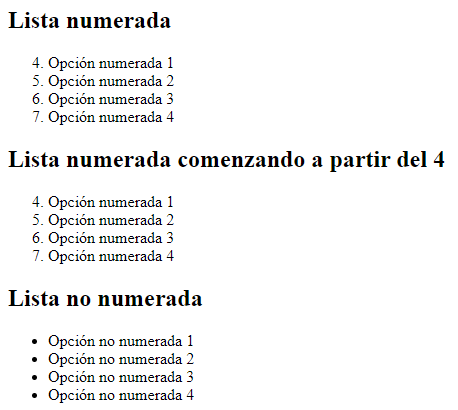
\includegraphics[height=8cm]{ss_html/listas.png}
\end{figure}

\textit{Nota}: este es el aspecto predeterminado de las listas en HTML, antes se le podía dar otro aspecto a ambos tipos de listas con un atributo \textit{type}, sin embargo, este ya no es utilizado, para sustituirlo, se recomienza personalizar o estilizar las listas con CSS.


\subsection{Tablas}
\hspace{0.55cm}La etiqueta \textbf{table} genera una tabla. Sus sub-etiquetas y atributos son:
\begin{itemize}
    \item \textbf{tr}: etiqueta que representa una fila en la tabla. Dentro de estas, va el contenido, celdas o columnas de cada fila.
    \item \textbf{td}: etiqueta que representa una celda, contenido o columna de una fila de una tabla.
    \item \textbf{th}: etiqueta que representa la cabecera o título de cada columna de una tabla.
    \item \textbf{colspan}: atributo que combina \textit{n} cantidad de columnas o celdas en una tabla.
    \item \textbf{rowspan}: atributo que combina \textit{n} cantidad de filas en una tabla.
    \item Los atributos \textit{align}, \textit{width} y \textit{height} aplican a las etiquetas \textbf{tr} y \textbf{td}.
    \item Los atributos \textit{width}, \textit{height}, \textit{bgcolor} y \textit{border} aplican a la esta etiqueta y a las sub-etiquetas.
\end{itemize}

Un ejemplo del aspecto de las tablas es el siguiente, junto con la \textit{Figura \ref{fig: 5}}:
\begin{lstlisting}
    <h2>Tabla regular</h2>
    <!-- Borde de 2 píxeles, ancho y alto de 200 píxeles. -->
    <table border="2px" width="200px" height="200px">
        <!-- Elementos alineados al centro. -->
        <tr align="center">
            <td>1</td>
            <td>2</td>
            <td>3</td>
        </tr>
        <tr align="center">
            <td>4</td>
            <td>5</td>
            <td>6</td>
        </tr>
        <tr align="center">
            <td>7</td>
            <td>8</td>
            <td>9</td>
        </tr>
    </table>
    <h2>Tabla con columnas combinadas</h2>
    <table border="2px" width="200px" height="200px">
        <tr align="center">
            <!-- Crea dos celdas que combinan dos columnas. -->
            <td colspan="2">1</td>
            <td colspan="2">2</td>
        </tr>
        <tr align="center">
            <td>3</td>
            <td>4</td>
            <td>5</td>
            <td>6</td>
        </tr>
        <tr align="center">
            <td>7</td>
            <td>8</td>
            <td>9</td>
            <td>10</td>
            </tr>
    </table>
    <h2>Tabla con filas combinadas</h2>
    <table border="2px" width="200px" height="200px">
        <tr align="center">
            <!-- Crea una fila que combina tres celdas. -->
            <td rowspan="3">1</td>
            <td>2</td>
            <td>3</td>
            <td>4</td>
        </tr>
        <tr align="center">
            <td>7</td>
            <td>5</td>
            <td>6</td>
        </tr>
        <tr align="center">
            <td>8</td>
            <td>9</td>
            <td>10</td>
        </tr>
    </table>
\end{lstlisting}
\begin{figure}[H]
    \centering
    \caption{Vista las Tablas}
    \label{fig: 5}
    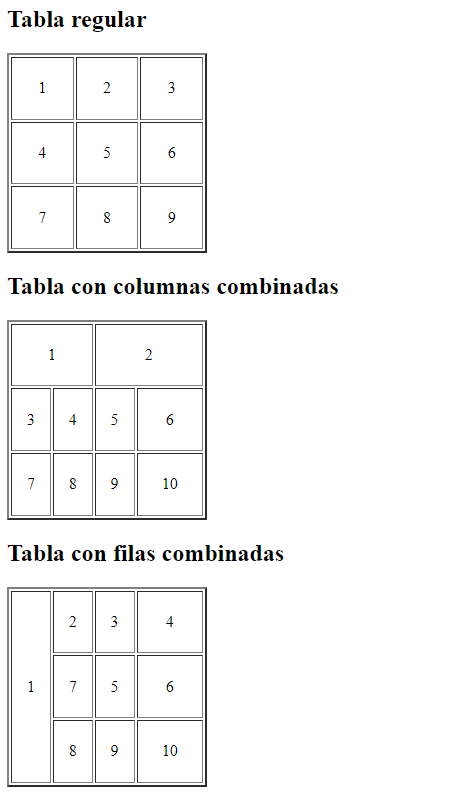
\includegraphics[height=12cm]{ss_html/tablas.png}
\end{figure}

Vemos que el ejemplo anterior posee tres tablas, con un borde de 2 píxeles, con todo su contenido alineado al centro y con un tamaño de ancho y alto de 200 píxeles, la primer tabla es una tabla regular de 3x3, la segunda tabla combina dos y dos columnas y la tercer tabla combina tres filas.


\subsection{Imágenes}
\hspace{0.55cm}Enlaza una imagen al sitio o página web con la etiqueta \textbf{img}. \textbf{Esta etiqueta no requiere una etiqueta de cierre}. Las imágenes son pesadas, es recomendado utilizar imágenes del tamaño que se deseen o requieran mostrar, ni tan grandes ni tan pequeñas, y en el formato adecuado (.jpg, .png u otros). Sus atributos son:
\begin{itemize}
    \item \textbf{src}: la ruta o dirección web de la imagen.
    \item \textbf{alt}: el texto o imagen alternativo en caso de que la imagen principal no cargue.
    \item Los atributos \textit{align}, \textit{height}, \textit{width} y \textit{border} aplican a esta etiqueta.
\end{itemize}

El uso de imágenes ya se vio en la Figura \ref{fig: 3}.


\subsection{Enlaces}
\hspace{0.55cm}Enlaza a un documento, imagen, archivo, sitio o página o dirección web con la etiqueta \textbf{a}. Sus atributos son:
\begin{itemize}
    \item \textbf{href}: es el enlace a donde se redireccionará.
    \item \textbf{target}: establece como dónde y cómo se abrirá el enlace o documento. Sus posibles valores son:
    \begin{itemize}
        \item \textbf{\_ blank}: carga en una nueva pestaña.
        \item \textbf{\_ self}: carga en el actual \textit{frame}.
        \item \textbf{\_ parent}: carga en el \textit{frame} padre o del \textit{frame} actual.
        \item \textbf{\_ top}: carga en la pestaña actual.
        \item \textbf{framename}: carga en un \textit{frame} determinado.
    \end{itemize}
    \item El atributo \textit{align} aplica a esta etiqueta.
\end{itemize}

Un ejemplo del aspecto de los enlaces es el siguiente, junto con la \textit{Figura \ref{fig: 6}}, donde se muestra el aspecto del enlace antes de dar clic en él, la \textit{Figura \ref{fig: 7}} muestra que se ha abierto otra pestaña después de haber dado clic en el enlace:
\begin{lstlisting}
    <a href="https://github.com/migueluisV" target="_blank">Github</a>
\end{lstlisting}
\begin{figure}[H]
    \centering
    \caption{Vista de Enlaces previo al clic}
    \label{fig: 6}
    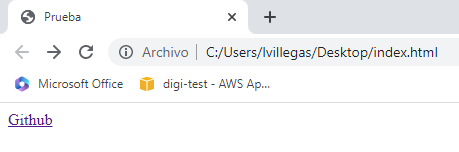
\includegraphics[width=11cm]{ss_html/enlaces_1.png}
\end{figure}
\begin{figure}[H]
    \centering
    \caption{Vista de Enlaces después del clic}
    \label{fig: 7}
    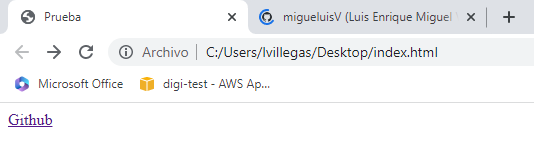
\includegraphics[width=11cm]{ss_html/enlaces_2.png}
\end{figure}

Al enlace se le configuró el atributo \textit{target} con el valor \textbf{\_ blank} para que se abriera el enlace en una nueva pestaña, puede probar con los otros valores de este atributo para ver el comportamiento.


\subsection{Formularios}
\hspace{0.55cm}La etiqueta \textbf{form} crea un formulario para recolectar información del usuario, esta información es enviada a un servidor u otro sitio o página, siendo procesada por un lenguaje de programación (PHP o JavaScript por ejemplo). Sus sub-etiquetas y atributos son:
\begin{itemize}
    \item \textbf{input}: etiqueta que crea un control para que el usuario interactúe con el. Sus atributos son:
    \begin{itemize}
        \item \textbf{type}: es el tipo de control a generar. Sus posibles valores son:
        \begin{itemize}
            \item \textbf{text}: caja de texto.
            \item \textbf{password}: caja de texto con caracteres especiales para proteger texto.
            \item \textbf{radio}: RadioButton.
            \item \textbf{checkbox}: caja de marcado.
            \item \textbf{submit}: botón que envía la información del formulario.
        \end{itemize}
        \item \textbf{placeholder}: texto por defecto que se muestra en una caja de texto.
        \item \textbf{name}: nombre único del control.
        \item \textbf{value}: el valor que almacena el control, se suele aplicar a \textit{submit}, \textit{radio} y \textit{checkbox}.
    \end{itemize}
    \item \textbf{textarea}: caja de texto multilínea. Tiene un inicio y final.
    \begin{itemize}
        \item \textbf{rows}: indica las filas por defecto de la textarea.
        \item \textbf{cols}: indica las columnas por defecto de la textarea.
        \item Los atributos \textit{name} y \textit{placeholder} aplican a esta etiqueta.
    \end{itemize}
    \item \textbf{action}: atributo de \textbf{form} que carga una dirección web una vez se llenó y envió el formulario. Si se le pone el valor \textbf{\#} a este atributo, el formulario cargará la página donde está contenido (se refrescará la página sin cambio alguno).
    \item \textbf{method}: atributo de \textbf{form} especifica el método HTTP cuando el formulario es enviado. Sus posibles valores son:
    \begin{itemize}
        \item \textbf{GET}: la información recolectada puede verse en la dirección web del sitio a donde fue mandada.
        \item \textbf{POST}: la información no es visible, y ofrece mejor seguridad si es que la información es sensible o se está actualizando.
    \end{itemize}
    \item Dependiendo de cómo se presente el formulario (con \textbf{div}, \textbf{span}, \textbf{p} u otros), se le pueden aplicar los atributos más populares anteriormente vistos.
\end{itemize}

Un ejemplo del aspecto de los enlaces es el siguiente, junto con la \textit{Figura \ref{fig: 8}}:
\begin{lstlisting}
    <form action="#" method="POST">
        p>Caja de texto: </p><input type="text" name="txt1" placeholder="Ingresa un texto..." />
        
        <p>Caja de texto multi línea: </p><textarea name="txta1" rows="10" cols="50" placeholder="Ingresa un texto..."></textarea>
        
        <p>Contraseña: </p><input type="password" name="psw1" />
        
        <p>RadioButtons: </p>
        <input type="radio" name="rb1" value="1" />Valor 1
        <br/>
        <input type="radio" name="rb1" value="2" />Valor 2
        
        <p>Checkbox: </p>
        <input type="checkbox" name="chb1" value="3" />Opción 1
        <br/>
        
        <input type="checkbox" name="chb2" value="4" />Opción 2
        
        <p>Botones: </p><input type="submit" name="btn1" value="Enviar" />
    </form>
\end{lstlisting}
\begin{figure}[H]
    \centering
    \caption{Vista de los Formularios}
    \label{fig: 8}
    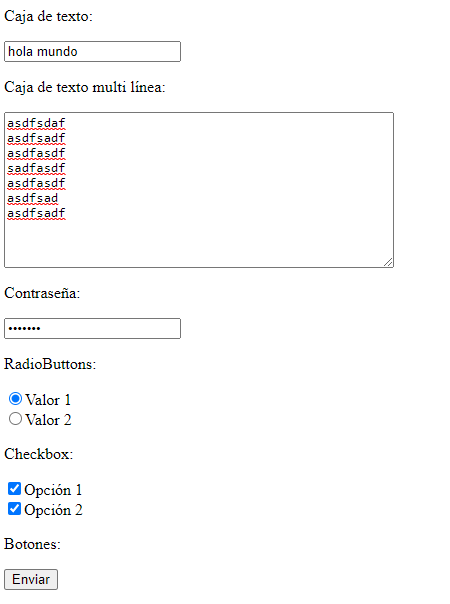
\includegraphics[height=12cm]{ss_html/formularios.png}
\end{figure}

Se creó un formulario con una caja de texto, una caja de texto multilínea, una caja para contraseñas, dos opciones de RadioButtons, dos opciones de CheckBoxs y un botón que envía la información recaba al mismo sitio. El formulario tiene el atributo \textit{action} y \textit{method} con los valores \textbf{\#} y \textbf{POST} respectivamente, envía la información protegida al mismo sitio donde está contenido el formulario. Algunas cajas de texto tienen el atributo \textit{placeholder}, para que se muestre un texto predeterminado que se elimina una vez el usuario ingresa algún texto. El control textarea posee los atributos \textit{rows} y \textit{cols} para mostrar una cantidad determinada de filas y columnas respectivamente, esto para resaltar que es un control multilínea.

Fíjese que el nombre de los dos RadioButtons utilizados es el mismo, esto es así ya que este control solo permite seleccionar una opción, si tuviéramos dos o más RadioButtons con distinto nombre, se podrían seleccionar todos sin problema; esto no ocurre con los CheckBoxs.

Todos los controles utilizados en el ejemplo anterior poseen su nombre único con el atributo \textit{name}; \textbf{existen más controles}.


\subsection{Frames}
\hspace{0.55cm}Los \textbf{frames} son contenedores donde podemos almacenar distintas páginas o contenido dentro de una sola ventana o página. El \textbf{frameset} es la etiqueta Block-Level de los \textbf{frames}, esta define cuantos frames habrá en el frameset (columnas y filas), su espacio definido, borde, etc.

Esta etiqueta o estructura ya no está soportada en HTML5. \textbf{frameset} sustituye la etiqueta \textbf{body} en un documento HTML. Algunos de sus atributos son:
\begin{itemize}
    \item \textbf{cols}: atributo que establece en cuántas columnas se seccionará la página web. El tamaño de estas columnas se determina por porcentajes o píxeles.
    \item \textbf{rows}: atributo que establece en cuántas filas se seccionará la página web. El tamaño de estas filas se determina por porcentajes o píxeles.
    \item \textbf{src}: atributo que determina el archivo o sitio web que se cargará en el frame.
    \item \textbf{noresize}: atributo que indica que un frame no puede cambiar su tamaño.
    \item \textbf{noframe}: etiqueta que indica al buscador que la página o sitio no soporta frames.
\end{itemize}

Veamos un ejemplo tomado de internet modificado por nosotros enseguida, en la \textit{Figura \ref{fig: 9}}:
\begin{lstlisting}
    <html>
        <head>
            <title>Un documento simple con marcos</title>
        </head>
        <frameset rows="20%,80%">
            <frameset cols="20%, 80%">
                <frame src="https://images.hola.com/imagenes/mascotas/20180925130054/consejos-para-cuidar-a-un-gatito-recien-nacido-cs/0-601-526/cuidardgatito-t.jpg">
                <frame src="https://images.unsplash.com/photo-1593288942460-e321b92a6cde?ixlib=rb-4.0.3&ixid=MnwxMjA3fDB8MHxleHBsb3JlLWZlZWR8Mnx8fGVufDB8fHx8&w=1000&q=80">
            </frameset>
            <frame src="https://images.unsplash.com/photo-1591871937631-2f64059d234f?ixlib=rb-4.0.3&ixid=MnwxMjA3fDB8MHxleHBsb3JlLWZlZWR8MXx8fGVufDB8fHx8&w=1000&q=80">
        </frameset>
    </html>
\end{lstlisting}
\begin{figure}[H]
    \centering
    \caption{Vista de los Framesets}
    \label{fig: 9}
    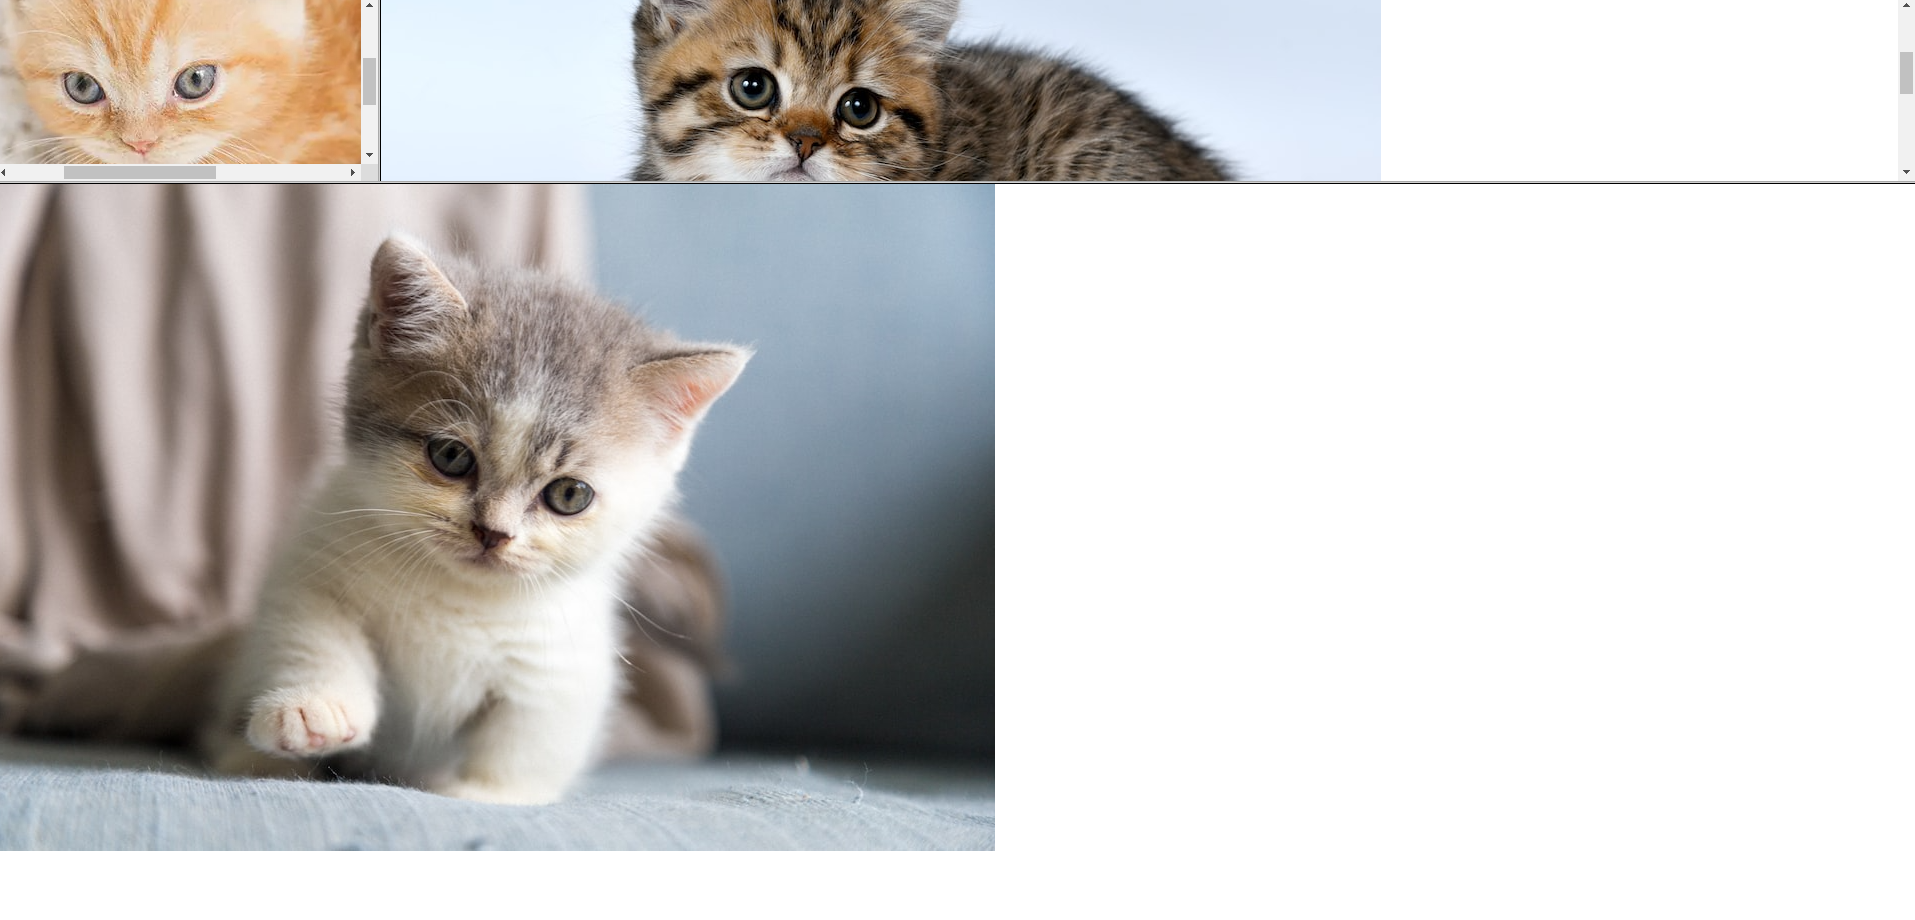
\includegraphics[width=13cm]{ss_html/frames_1.png}
\end{figure}

El ejemplo presenta un \textbf{frameset} principal que contiene dos columnas, una del tamaño del 20\% de la pantalla y la otra del 80\%: el primer \textbf{frame} contiene otro \textit{frameset} con dos filas, igual con tamaños de 20 y 80 porciento, así combinamos el uso de framesets. El principal pose un borde de 3 píxeles, que afecta al resto de frames o framesets internos, vemos que aquellos que requieren de desplazamiento se les inserta automáticamente barras deslizadoras para recorrer el frame, si ponemos el puntero en los bordes, estos pueden ser redimensionados, como se ve en la \textit{Figura \ref{fig: 10}}:
\begin{figure}[H]
    \begin{center}
        \caption{Vista de los Framesets redimensionados}
        \label{fig: 10}
        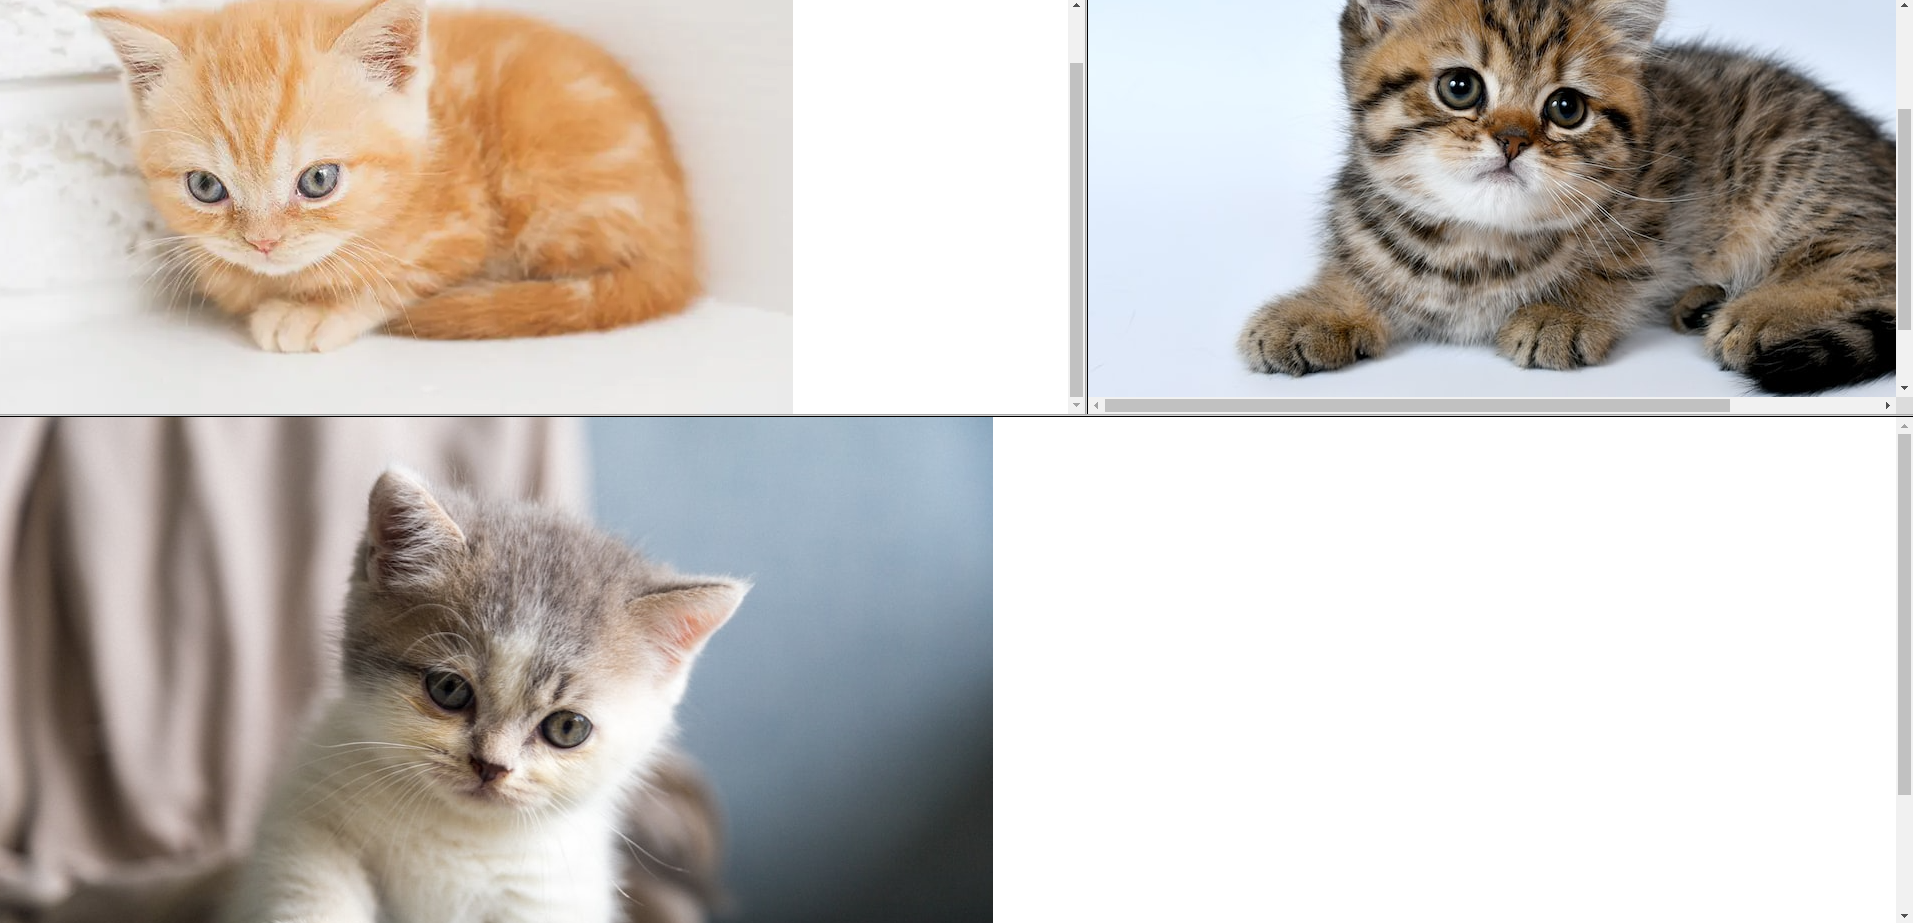
\includegraphics[width=13cm]{ss_html/frames_2.png}
    \end{center}
\end{figure}

En caso de que no se requiera la posibilidad de redimensionamiento de frames, aplicar el atributo \textit{noresize}. \textbf{frameset ya no es soportado por HTML5}.


\subsection{Colores}
\hspace{0.55cm}Los colores son representados como valores hexadecimales:
\begin{center}
    0, 1, 2, 3, 4, 5, 6, 7, 8, 9, A, B, C, D, E, F
\end{center}

Los colores en HTML son desplegados según el modelo RGB (Red, Green, Blue), para escribir un color es necesario escribir el símbolo de gato (\#), seguido de su código de combinación de tres o seis, como vemos el la \textit{Figura \ref{fig: 11}}:
\begin{figure}[H]
    \centering
    \caption{Ejemplo de colores HTML}
    \label{fig: 11}
    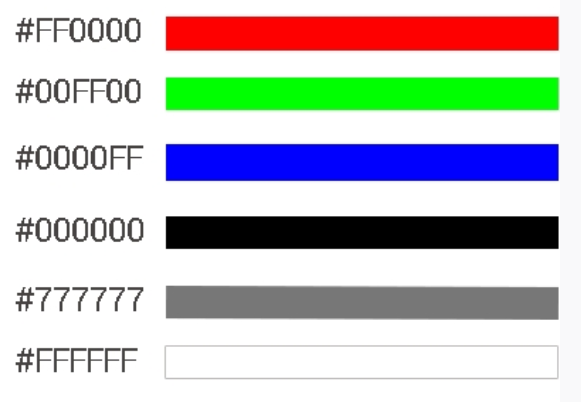
\includegraphics[width=7cm]{ss_html/ejemplo_colores.png}
\end{figure}
\section{HTML5}
\hspace{0.55cm}Algunas de las nuevas características que incluye la versión más reciente de HTML son los formularios 2.0, que traen controles para seleccionar fechas, colores, números, cajas de texto para correos electrónicos, búsqueda, URL, los métodos PUT y DELETE, entre otros; el tipo de documento previo al inicio de la estructura HTML, nuevas etiquetas, la posibilidad de modificar la codificación de caracteres, entre otros temas que se verán en este documento.


\subsection{Modelos de contenido}
\hspace{0.55cm}Los \textbf{modelos de contenido} son modelos de etiquetas que responden a una misma función o que tienen un fin determinado, los modelos pueden ir enfocados a la interacción, la organización, inserción, formateo o adición de información de una página o sitio web. Estos modelos suelen contener ciertas etiquetas que responden al fin del mismo.

Anteriormente, habíamos mencionado que HTML tenía etiquetas Block-Level e Inline, donde la segunda suele pertenecer a la primera (revisar la sección \textbf{Tipos de elementos}), en esta versión del lenguaje, se agregan siete modelos nuevos:
\begin{enumerate}
    \item Metadata: establece información adicional o comportamiento al resto del contenido de la página o sitio. Podemos encontrar las siguientes etiquetas en este modelo: \textbf{base}, \textbf{link}, \textbf{meta}, \textbf{noscript}, \textbf{script}, \textbf{style}, \textbf{title}.
    \item Embedded: contenido que es importado a la estructura o contenido de la página o sitio. Podemos encontrar las siguientes etiquetas en este modelo: \textbf{audio}, \textbf{video}, \textbf{canvas}, \textbf{iframe}, \textbf{img}, \textbf{math}, \textbf{object}, \textbf{svg}.
    \item Interactive: contenido hecho para que el usuario interactue con él. Podemos encontrar las siguientes etiquetas en este modelo: \textbf{a}, \textbf{audio}, \textbf{video}, \textbf{button}, \textbf{details}, \textbf{embed}, \textbf{iframe}, \textbf{img}, \textbf{input}, \textbf{label}, \textbf{object}, \textbf{select}, \textbf{textarea}.
    \item Heading: establece cabeceras o secciones en el documento. Podemos encontrar las siguientes etiquetas en este modelo: \textbf{h1} a \textbf{h6} y \textbf{hgroup}.
    \item Phrasing: es un modelo para formatear contenido, posee varias etiquetas compartidas con HTML4: \textbf{img}, \textbf{span}, \textbf{strong}, \textbf{label}, \textbf{br/}, \textbf{small}, \textbf{sub} y más.
    \item Flow: contiene la mayoría de las etiquetas que serán utilizadas en la estructura, flujo o funcionamiento del documento. Se puede decir que este modelo incluye la mayoría del resto.
    \item Sectioning: establece el objetivo de las secciones, contenido, navegación o pies de páginas. Podemos encontrar las siguientes etiquetas en este modelo: \textbf{article}, \textbf{aside}, \textbf{nav}, \textbf{section}.
\end{enumerate}

La \textit{Figura \ref{fig: 12}} nos muestra un diagrama de como se relacionan estos modelos:
\begin{figure}[H]
    \centering
    \caption{Relación de los modelos de contenido HTML5}
    \label{fig: 12}
    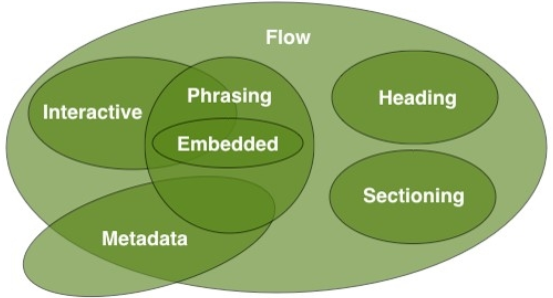
\includegraphics[width=9cm]{ss_html/modelos.png}
\end{figure}

Ojo, no es como que tengamos que escoger un modelo para desarrollar nuestro proyecto, simplemente son contenedores de etiquetas que tienen un fin específico.


\subsection{Estructura de páginas HTML5}
\hspace{0.55cm}La estructura básica o más simple de un sitio web moderno HTML5 se aprecia en la \textit{Figura \ref{fig: 13}} (no es necesario que se agreguen todas las secciones de esta estructura):
\begin{figure}[H]
    \centering
    \caption{Estructura básica de un sitio web HTML5}
    \label{fig: 13}
    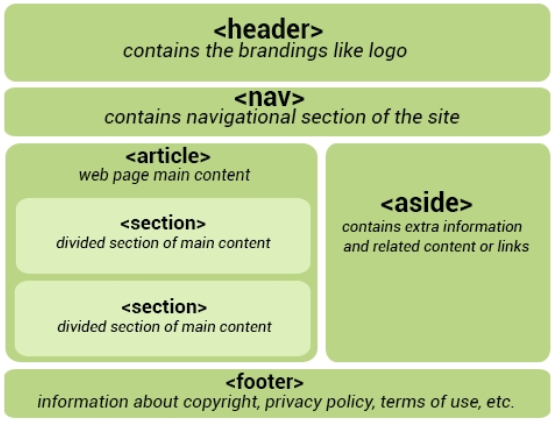
\includegraphics[width=9cm]{ss_html/estructura basica_html5.png}
\end{figure}


\subsubsection{headers, nav y footer}
\hspace{0.55cm}La etiqueta \textbf{header} es la cabecera del sitio, donde está el logo del sitio o información más importante del sitio, si queríamos crear un \textit{header} con HTML4, debíamos utilizar un contenedor \textbf{div}:
\begin{center}
    \textit{$<$div id="header"$>$}
\end{center}

Con HTML5, poseemos la etiqueta \textbf{header} que vuelve más fácil esta tarea:
\begin{lstlisting}
    <!-- Cabecera del sitio. -->
    <header>
	<h1>Nombre y logo del sitio</h1>
    </header>
    <!-- Resto del sitio. -->
    <h3>Esto es el cuerpo del sitio</h3>
    <h3>Esto es el cuerpo del sitio</h3>
    <h3>Esto es el cuerpo del sitio</h3>
\end{lstlisting}

La etiqueta \textbf{nav} es un menú horizontal que te permite navegar a lo largo de todo el sitio web, por lo que \textit{nav} está constituido de enlaces:
\begin{lstlisting}
    <!-- Cabecera del sitio. -->
    <header>
        <h1>Nombre y logo del sitio</h1>
    </header>
    <!-- Barra de navegación del sitio. -->
    <nav>
        <ul>
            <li><a href="#">Home</a></li>
            <li><a href="#">Servicios</a></li>
            <li><a href="#">Acerca de nosotros</a></li>
            <li><a href="#">Organigrama</a></li>
        </ul>
    </nav>
    <!-- Resto del sitio. -->
    <h3>Esto es el cuerpo del sitio</h3>
    <h3>Esto es el cuerpo del sitio</h3>
    <h3>Esto es el cuerpo del sitio</h3>
\end{lstlisting}


La etiqueta \textbf{footer} es el pie de página del sitio o página, nos permite poner información hasta abajo de la página: este tipo de información suele ser la información de contacto, política de privacidad, redes sociales, términos de uso, información de Copyright, documentos relacionados, mapa del sitio, etc:
\begin{lstlisting}
    <!-- Cabecera del sitio. -->
    <header>
        <h1>Nombre y logo del sitio</h1>
    </header>
    <!-- Barra de navegación del sitio. -->
    <nav>
        <ul>
            <li><a href="#">Home</a></li>
            <li><a href="#">Servicios</a></li>
            <li><a href="#">Acerca de nosotros</a></li>
            <li><a href="#">Organigrama</a></li>
        </ul>
    </nav>
    <!-- Cuerpo del sitio. -->
    <h3>Esto es el cuerpo del sitio</h3>
    <h3>Esto es el cuerpo del sitio</h3>
    <h3>Esto es el cuerpo del sitio</h3>
    <!-- Pie del sitio. -->
    <footer>
        <h3>Mapa del sitio/h3>
    </footer>
\end{lstlisting}

La \textit{Figura \ref{fig: 14}} muestra el resultado de los dos ejemplos anteriores:
\begin{figure}[H]
    \centering
    \caption{Ejemplo de header y footer}
    \label{fig: 14}
    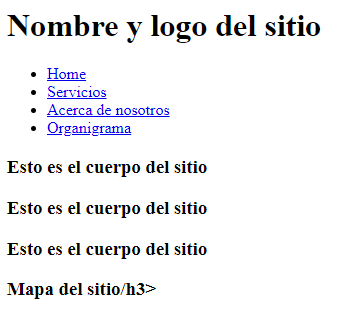
\includegraphics[width=7cm]{ss_html/header_footer.png}
\end{figure}

\textit{Nota}: el buscador ya tiene definido la información de la cabecera, menú de navegación y pie de página, aunque visualmente no parezca nada relevante.


\subsubsection{article, section y aside}
\hspace{0.55cm}La etiqueta \textbf{article} representa un contenedor para un artículo, foro, post, revista, artículo de periódico, entrada de blog, un comentario, un \textit{widget} o \textit{gadget} interactivo u otro elemento independiente del contenido del sitio, las etiquetas \textit{article} pueden ser anidadas unas dentro de otras, y estos contenedores deben ser independiente al resto del contenido de la página o sitio web. Veamos el siguiente ejemplo:
\begin{lstlisting}
    <article>
        <article>
            <h2>Nombre del artículo</h2>
            <h1>Autor</h1>
        </article>
        <article>
            <h4>Fecha de publicación</h4>
            <h4>Sitio de publicación</h4>
        </article>
        <article>
            <p>Contenido del artículo</p>
        </article>
    </article>
\end{lstlisting}

Anidamos etiquetas \textit{article} dentro de una etiqueta mayor \textit{article}, esto con el fin de que cada etiqueta anidada sea un dato o sección propiamente de un artículo que se esté insertando al documento HTML.

La etiqueta \textbf{section} es un contenedor para diversas etiquetas HTML, estas etiquetas contenidas deben tener algo en común, y es que deben pertenecer a una sección de la página o sitio web; algunas etiquetas que pueden ser utilizadas en las secciones son: \textbf{h1-h6}, \textbf{p}, otra etiqueta \textbf{section} o \textbf{article}. Veamos el siguiente ejemplo:
\begin{lstlisting}
    <article>
        <section>
            <h2>Nombre del artículo</h2>
            <h1>Autor</h1>
        </section>
        <section>
            <h4>Fecha de publicación</h4>
            <h4>Sitio de publicación</h4>
        </section>
        <section>
            <p>Contenido del artículo</p>
        </section>
    </article>
\end{lstlisting}

Se sustituyen los \textit{articles} anidados por \textit{sections}. La diferencia entre article y section es que, article va enfocado contener contenido independiente del sitio web, mientras que section puede contener otros artículos o secciones del propio sitio web.

La etiqueta \textbf{aside} representa contenido relacionado a otro contenido, pudiendo ser este de una etiqueta \textit{article}, de un \textit{section} o del propio sitio web. Veamos un ejemplo:
\begin{lstlisting}
    <article>
        <article>
            <h2>Nombre del artículo</h2>
            <h1>Autor</h1>
        </article>
        <article>
            <h4>Fecha de publicación</h4>
            <h4>Sitio de publicación</h4>
        </article>
        <article>
            <p>Contenido del artículo</p>
        </article>
        <aside>
            <a href="#">Vea estos otros artículos similares</a>
        </aside>
    </article>
\end{lstlisting}

Si copia algunos de los ejemplos anteriores y lo ejecuta en el navegador de su preferencia, verá un sitio bastante sencillo ni diseño particular, pero para el buscador, la existencia de una etiqueta \textit{article}, \textit{section} o \textit{aside} le permitirá una estructuración determinada del sitio.


\subsubsection{\textit{div}, \textit{class} e \textit{id} vs la estructura HTML5}
\hspace{0.55cm}Veamos sus diferencias:
\begin{itemize}
    \item \textbf{div, class e id}: contenedores de uso muy general, utilizados para contener etiquetas HTML y aplicarles un estilo o evento.
    \item \textbf{article}: contenedor de uso muy específico, para contenido independiente al del sitio o página web.
    \item \textbf{section}: contenedor de uso general, utilizado para contener otras etiquetas \textit{article} o HTML, pero que tengan una relación entre sí.
    \item \textbf{aside}: contenedor para contenido secundario relacionado con respecto a otro.
\end{itemize}
\subsection{APIs}


\subsubsection{Web Storage}

El almacenamiento web de HTML5 permite guardar información y datos en la computadora del usuario que acceda a nuestro sitio y genera datos, con esto, podemos acceder a ellos si es que el usuario entra en otro momento, evitamos enviar la información nuevamente (si es que ya fue almacenada), tomarla si ya fue almacenada, es más seguro, etc. Para utilizar esta API, es necesario conocer JavaScript.

\textbf{Tipos del almacenamiento web.}

\begin{itemize}
    \item \textbf{sessionStorage()}: crea una sesión y almacena información en la misma; esta información y sesión serán destruidas una vez el usuario cierre el buscador.
    \item \textbf{localStorage()}: crea una sesión sin expiración y almacena la información en la máquina del usuario.
\end{itemize}

\textbf{Operaciones con el almacenamiento web.}

Todas estas operaciones son trabajadas con JavaScript, ya sea con un almacenamiento local o de sesión, los datos son almacenados por medio de un \textbf{par llave/valor}:
\begin{lstlisting}
    // Guardando datos.
    localStorage.setItem("llave1", "valor1");
    sessionStorage.setItem("llave1", "valor1");

    // Obteniendo e imprimendo datos guardados.
    alert(localStorage.getItem("llave1"));
    alert(sessionStorage.getItem("llave1"));

    // Eliminando un dato.
    localStorage.removeItem("llave1");
    sessionStorage.removeItem("llave1");

    // Eliminando todos los datos.
    localStorage.clear();
    sessionStorage.clear();
\end{lstlisting}


\subsubsection{Geolocation}

Es la ubicación actual del usuario (siendo más precisa en dispositivos con GPS), este dato compromete la privacidad de los individuos, por lo que el sitio web debe preguntar al usuario si este desea compartir su ubicación:
\begin{center}
    \textit{navigator.geolocation.getCurrentPosition();}
\end{center}

Donde los parámetros de \textit{getCurrentPosition()} son:
\begin{itemize}
    \item \textbf{showLocation}: obligatorio, establece un método que recibe la información de la ubicación.
    \item \textbf{ErrorHandler}: opcional, establece un método en caso de que un error ocurra en la llamada asíncrona.
    \item \textbf{Options}: opcional, define algunas opciones a la hora de recibir la información de la ubicación.
\end{itemize}

\textbf{Presentando la información}

La información de la ubicación puede ser presentada en las siguientes formas:
\begin{itemize}
    \item \textbf{Geodetic}: es presentada según latitud y longitud.
    \item \textbf{Civic}: es presentada de una manera más simple para una persona, por medio de ciudades y otros datos civiles.
\end{itemize}

La \textit{Figura \ref{fig: 18}} lo explica mejor:
\begin{figure}[H]
    \centering
    \caption{Formas de presentar la geolocalización}
    \label{fig: 18}
    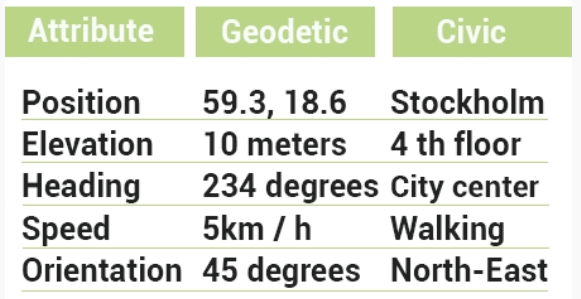
\includegraphics[width=7cm]{ss_html/geolocation.png}
\end{figure}

\textit{Nota}: el método \textbf{getCurrentPosition()} siempre regresa un objeto, donde los atributos \textit{latitude}, \textit{longitude} y \textit{accuracy} siempre son retornados.

El siguiente ejemplo nos ayudará a comprender la forma de trabajar la geolocalización (\textit{Figura \ref{fig: 19}}):
\begin{lstlisting}
    <p>Click the button to get your coordinates.</p>
    <!-- Botón que al presionarlo llama a la función "getLocation" del script insertado. -->
    <button onclick="getLocation()">Try It</button>
            
    <p id="demo"></p>

    <script>
        var x = document.getElementById("demo");

        // Obtiene la localización del buscador.
        function getLocation() {
            if (navigator.geolocation) {
                navigator.geolocation.getCurrentPosition(showPosition);
            }
            else { 
                x.innerHTML = "Geolocation is not supported by this browser.";
            }
        }
        // Muestra la localización en HTML.
        function showPosition(position) {
            x.innerHTML = "Latitude: " + position.coords.latitude + 
            "<br>Longitude: " + position.coords.longitude;
        }
    </script>
\end{lstlisting}
\begin{figure}[H]
    \centering
    \caption{Ejemplo de geolocalización}
    \label{fig: 19}
    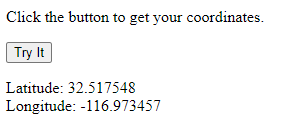
\includegraphics[width=7cm]{ss_html/geolocation_1.png}
\end{figure}


\subsubsection{Drag \& Drop}

Todos las etiquetas y objetos HTML pueden ser \textit{draggable}, solamente añada el atributo \textbf{draggable} con su valor \textbf{true}:
\begin{center}
    \textit{$<$img draggable="true" /$>$}
\end{center}

Esto es por parte de HTML, la API del Drag \& Drop está basada en un evento JavaScript, como vemos en el siguiente ejemplo:
\begin{lstlisting}
    <html>
        <head>
            <!-- Script interno. -->
            <script>
                // Permite el arrastrado de etiquetas.
                function allowDrop(ev) {
                    ev.preventDefault();
                }
                // Realiza la acción de arrastrar la etiqueta y su información.
                function drag(ev) {
                    ev.dataTransfer.setData("text", ev.target.id);
                }
                // Realiza la acción de soltar la etiqueta y su información.
                function drop(ev) {
                    ev.preventDefault();
                    var data = ev.dataTransfer.getData("text");
                    ev.target.appendChild(document.getElementById(data));
                }
            </script>
        </head>
        <body>
            <!-- Establece contenedor para soltar un elemento. -->
            <div id="box" ondrop="drop(event)" ondragover="allowDrop(event)"
                style="border:1px solid black; width:200px; height:200px">
            </div>
            <!-- Etiqueta capaz de ser arrastrada. -->
            <img id="image" src="sample.jpg" draggable="true"
                ondragstart="drag(event)" width="150" height="50" alt="" />
        </body>
    </html>
\end{lstlisting}

La explicación es la siguiente: cuando una etiqueta u objeto es arrastrado (dragged), el atributo \textbf{ondragstart} llama a una función: \textbf{drag(event)}, el cual especifica la información a arrastrar. El método \textbf{dataTransfer.setData()} especifica el tipo y valores de la información arrastrada; este método te permite acceder también a la información del objeto o etiqueta arrastrada, regresará cualquier información asignada al tipo dado en el método \textbf{setData()}, este tipo puede ser el ID del elemento arrastrado (imágenes, videos, audios, paneles, etc).

El evento \textbf{ondragover} especifica dónde la información puede ser soltada. Por defecto, la información o etiquetas no pueden ser soltadas sobre otras etiquetas, por lo que debemos prevenir esto mediante el método \textbf{preventDefault()}; permite prevenir al buscador que se cambiará la forma por defecto para manejar la información (\textit{por defecto está como enlace a soltar, no otros objetos}).

Al soltar el clic y soltar (drop) la etiqueta, objeto o información, ocurre el evento \textit{drop}. El atributo \textbf{ondrop} va ligado al objeto que recibirá lo que sea que se le suelte, a quien recibirá la información u objeto.


\subsection{SVG}

SVG significa \textbf{Scalable Vector Graphics} (Gráficos vectoriales escalables), y es utilizado para dibujar figuras con un estilo HTML. En HTML funciona tanto como una etiqueta, como en un formato de imagen para una etiqueta \textit{img}, y la podemos utilizar para dibujar cajas, líneas, círculos, textos y gráficas en imágenes (recordemos que los formatos \textit{.svg} puede ser aumentada o disminuida de tamaño sin perder calidad).
\begin{center}
    \textit{$<$img src="imagen.svg" alt="" height="300" /$>$}
\end{center}

La etiqueta \textbf{svg} debe tener los atributos \textit{width} y \textit{height} de manera obligatoria, para dimensionar el panel o espacio donde será dibujada la figura; tome en cuenta que, si este espacio de dibujo es menor al tamaño de la figura, esta se dibujará incompleta en el espacio de dibujo.


\subsubsection{Dibujando figuras}

Crearemos un \textbf{círculo} en el siguiente ejemplo con su visualización (\textit{Figura \ref{fig: 20}}):
\begin{lstlisting}
    <!-- Crea un panel de dibujo SVG de 3000x3000 píxeles. -->
    <svg width="3000" height="3000">
        <!-- Dibuja un círculo de radio 50, de color rojo y borde negro.. -->
        <circle cx="100" cy="150" r="50" fill="red" stroke="black"/>
    </svg>
\end{lstlisting}
\begin{figure}[H]
    \centering
    \caption{Dibujando un círculo con SVG}
    \label{fig: 20}
    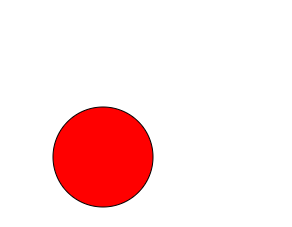
\includegraphics[width=7cm]{ss_html/svg_circle.png}
\end{figure}

Donde:
\begin{itemize}
    \item \textbf{cx}: coordenada \textit{x}, empuja el centro del círculo desde la izquierda de la página.
    \item \textbf{cy}: coordenada \textit{y}, empuja el centro del círculo desde la parte superior de la página.
    \item \textbf{r}: radio del círculo.
    \item \textbf{fill}: rellena la figura con un color.
    \item \textbf{stroke}: añade un borde de color a la figura (atributo más personalizable en CSS).
\end{itemize}

Como podemos suponer, hay ciertos atributos únicos para cada figura posible para dibujar, otros son más generales, como \textit{fill} o \textit{stroke}.

Ahora crearemos un \textbf{rectángulo} en el siguiente ejemplo con su visualización (\textit{Figura \ref{fig: 21}}):
\begin{lstlisting}
    <svg width="3000" height="3000">
        <!-- Dibuja un rectángulo de 300x100 píxeles, de color rojo y borde negro. -->
        <rect width="300" height="100" x="30" y="30" fill="red" stroke="black" />
    </svg>
\end{lstlisting}
\begin{figure}[H]
    \centering
    \caption{Dibujando un rectángulo con SVG}
    \label{fig: 21}
    
\includegraphics[width=7cm]{ss_html/svg_rect.png}
\end{figure}

Donde:
\begin{itemize}
    \item \textbf{width}: ancho del rectángulo.
    \item \textbf{height}: altura del rectángulo.
    \item \textbf{x}: coordenada \textit{x}, igual que el atributo \textit{cx}.
    \item \textbf{y}: coordenada \textit{y}, igual que el atributo \textit{cy}.
\end{itemize}

Una \textbf{línea} puede ser dibujada siguiendo el ejemplo a continuación, el resultado puede apreciarse en la \textit{Figura \ref{fig: 22}}:
\begin{lstlisting}
    <svg width="3000" height="3000">
        <!-- Dibuja una línea negra con inicio en x(10,10) y y(200,100). -->
        <line x1="10" y1="10" x2="200" y2="100" stroke="black" />
    </svg>
\end{lstlisting}
\begin{figure}[H]
    \centering
    \caption{Dibujando una línea con SVG}
    \label{fig: 22}
    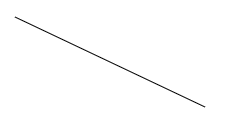
\includegraphics[width=7cm]{ss_html/svg_line.png}
\end{figure}

Donde:
\begin{itemize}
    \item \textbf{x1}: coordenada \textit{x} para el punto inicial de la línea, empuja este punto desde la izquierda de la página.
    \item \textbf{y1}: coordenada \textit{y} para el punto inicial de la línea, empuja este punto desde la parte superior de la página.
    \item \textbf{x2}: coordenada \textit{x} para el punto terminal de la línea, empuja este punto desde la izquierda de la página.
    \item \textbf{y2}: coordenada \textit{y} para el punto terminal de la línea, empuja este punto desde la parte superior de la página.
\end{itemize}

Una \textbf{polilínea} (una línea tras otra) puede ser dibujada siguiendo el ejemplo a continuación, el resultado puede apreciarse en la \textit{Figura \ref{fig: 23}}:
\begin{lstlisting}
    <svg width="3000" height="3000">
        <!-- Dibuja un camino de líneas que forman dos triángulos uno al lado del -->
        <!-- otro con relleno negro. -->
        <polyline points="100 100, 150 150, 200 100, 250 150, 300 100" stroke="black" />
    </svg>
\end{lstlisting}
\begin{figure}[H]
    \centering
    \caption{Dibujando una ruta con SVG}
    \label{fig: 23}
    
\includegraphics[width=7cm]{ss_html/svg_polyline.png}
\end{figure}

Donde:
\begin{itemize}
    \item \textbf{points}: son las coordenadas \textit{x}, \textit{y} de los puntos que seguirá la ruta, se separan únicamente por comas.
    \item \textbf{stroke}: en este caso, el atributo colorea por completo la ruta.
\end{itemize}

Una \textbf{elipse} puede ser dibujada siguiendo el ejemplo a continuación, el resultado puede apreciarse en la \textit{Figura \ref{fig: 24}}:
\begin{lstlisting}
    <svg width="3000" height="3000">
        <!-- Dibuja una elipse roja con borde negro. -->
        <ellipse cx="200" cy="100" rx="150" ry="70" fill="red" stroke="black" />
    </svg>
\end{lstlisting}
\begin{figure}[H]
    \centering
    \caption{Dibujando una elipse con SVG}
    \label{fig: 24}
    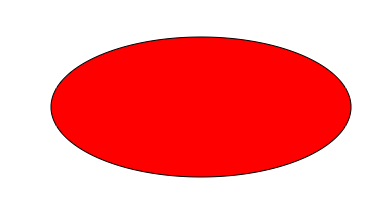
\includegraphics[width=7cm]{ss_html/svg_ellipse.png}
\end{figure}

Donde:
\begin{itemize}
    \item \textbf{cx}: coordenada \textit{x}, aplicable igual al círculo.
    \item \textbf{cy}: coordenada \textit{y}, aplicable igual al círculo.
    \item \textbf{rx}: tamaño del radio horizontal de la elipse.
    \item \textbf{ry}: tamaño del radio vertical de la elipse.
\end{itemize}

Un \textbf{polígono} puede ser dibujada siguiendo el ejemplo a continuación, el resultado puede apreciarse en la \textit{Figura \ref{fig: 25}}:
\begin{lstlisting}
    <svg width="3000" height="3000">
        <!-- Dibuja un polígono rojo con borde negro. -->
        <polygon points="100 100, 200 200, 300 0" fill="red" stroke="black" />
    </svg>
\end{lstlisting}
\begin{figure}[H]
    \centering
    \caption{Dibujando un polígono con SVG}
    \label{fig: 25}
    
\includegraphics[width=7cm]{ss_html/svg_polygon.png}
\end{figure}

Donde:
\begin{itemize}
    \item \textbf{points}: son las coordenadas \textit{x}, \textit{y} de los puntos que seguirá la ruta, se separan únicamente por comas.
\end{itemize}

\textit{Nota}: recuerde que el atributo \textit{stroke} puede ser modificado y personalizado a profundidad con CSS, al igual que el atributo \textit{fill}.


\subsubsection{Animaciones y rutas}

Además de crear figuras, svg puede crear animaciones con la etiqueta \textbf{animate} y sus siguientes atributos:
\begin{itemize}
    \item \textbf{attributeName}: especifica el atributo o variable que será afectada por la animación. Los valores que se le pueden dar a este atributo pueden ser: x, y, rx, ry, cx, cy, r, etc.
    \item \textbf{from}: valor inicial del atributo de la animación.
    \item \textbf{to}: valor final del atributo de la animación.
    \item \textbf{dur}: duración de la animación (3s, 4s, 10s).
    \item \textbf{fill}: indica qué ocurre con el valor del atributo o variable cuando la animación termina. Puede adoptar el valor "freeze" (mantiene el valor final que tuvo el atributo) o "remove" (resetea el valor del atributo).
    \item \textbf{repeatCount}: número de veces que se repetirá la animación. Puede utilizar el valor "indefinite" para que la animación se repita indefinidamente.
\end{itemize}

Pondremos un ejemplo donde un cuadrado baja infinitamente a continuación y puede ejecutarlo en su buscador:
\begin{lstlisting}
    <svg width="1000" height="1000">
        <rect width="150" height="150" fill="orange" stroke="black">
            <animate attributeName="y" from="0" to="300" dur="3s" fill="freeze" repeatCount="indefinite"/> 
        </rect>
    </svg>
\end{lstlisting}

Una \textbf{ruta} puede ser definida con la etiqueta \textbf{path}, su atributo \textbf{d} es la que establece cómo será la ruta; al igual que el dibujado de figuras en la sección anterior, se utilizan coordenadas \textit{x}, \textit{y}, sin embargo, el atributo \textbf{d} puede contener valores adicionales a las coordenadas:
\begin{itemize}
    \item \textbf{M}: move to (punto inicial de la ruta).
    \item \textbf{L}: line to (línea diagonal, horizontal o vertical).
    \item \textbf{H}: horizontal line to.
    \item \textbf{V}: vertical line to
    \item \textbf{C}: curve to.
    \item \textbf{S}: smooth curve to.
    \item \textbf{Q}: quadratic Bézier curve.
    \item \textbf{T}: smooth quadratic Bézier curve to.
    \item \textbf{A}: elliptical Arc.
    \item \textbf{Z}: close path (cierra la ruta).
\end{itemize}

Como puede ver, estos valores adicionales están en mayúsculas, esto indica que la ruta tendrá una \textbf{posición absoluta}, si utiliza letras minúsculas la \textbf{posición será relativa}.

Creamos una ruta triangular a continuación, puede ver el resultado en la \textit{Figura \ref{fig: 26}}:
\begin{lstlisting}
    <svg width="3000" height="3000">
        <!-- Dibuja una ruta color negro. -->
   	<path d="M 0 0 L200 200 L400 0 Z" stroke="black" fill="none" />
    </svg>
\end{lstlisting}
\begin{figure}[H]
    \centering
    \caption{Dibujando una ruta con SVG y path}
    \label{fig: 26}
    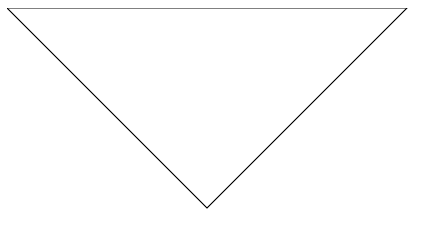
\includegraphics[width=7cm]{ss_html/svg_path.png}
\end{figure}

Nuestra área de dibujo debe tener un punto de inicio para dibujar la ruta, \textit{M 0 0} crea este punto de inicio, \textit{L200 200} crea una línea entre las coordenadas (0, 0) y (200, 200), \textit{L400 0} crea una línea entre las coordenadas (200, 200) y (400, 0), finalmente, \textit{Z} dibuja una línea entre el último punto creado (400, 0) y el punto inicial (0, 0); de esta manera, podemos conseguir crear rutas en nuestros documentos HTML. Nótese que el atributo \textit{fill} tiene el valor \textbf{none}, esto evita que la ruta se coloree completamente (cosa que ocurrió dibujando polilíneas).

\subsection{Canvas}

La etiqueta \textbf{canvas} es un contenedor para figuras o gráficos un poco más especializados o complejos, a diferencia de \textit{svg}, es necesario un script (JavaScript suele ser utilizado) para dibujar dentro de este contenedor.
\begin{center}
    \textit{$<$canvas id="canvas1" width="200" height="200"$>$$<$canvas$/>$}
\end{center}

El atributo \textit{id} se hace presente, porque es necesario para pasárselo al script, que le regresará un gráfico al contenedor canvas:
\begin{lstlisting}
    <!-- Crea un panel de dibujo Canvas de 400x300 píxeles. -->
    <canvas id="canvas1" width="400" height="300"></canvas> 

    <script>
        // Asigna a una variable el contenedor con id "canvas1".
        var can = document.getElementById("canvas1"); 
        // Establece el tipo de dibujo en 2D.
        var ctx = can.getContext("2d");
    </script>
\end{lstlisting}

Al igual que en svg, las coordenadas que maneja canvas son \textit{x}, \textit{y}, cada una de ellas empujan el gráfico insertado igual que como ocurre en svg (de izquierda a derecha y de superior a inferior en la página). Al igual que con svg, existen métodos de JS para dibujar figuras y pasárselos al canvas.

El método \textbf{fillRect(x, y, w, h)} dibuja un cuadrado o rectángulo rellenado (obligado) de color negro (por defecto), podemos suponer que los parámetros representan las coordenadas y dimensiones de la figura respectivamente. Pongamos un ejemplo y su resultado (\textit{Figura \ref{fig: 27}}):
\begin{lstlisting}
    <canvas id="canvas1" width="900" height="900"></canvas>
        
    <script>
        var c=document.getElementById("canvas1");
        var ctx=c.getContext("2d");
        // Dibuja un cuadrado con origen en (30,30) de 200x200 píxeles.
        ctx.fillRect(30,30,200,200);
    </script>
\end{lstlisting}
\begin{figure}[H]
    \centering
    \caption{Dibujando un cuadrado con Canvas}
    \label{fig: 27}
    
\includegraphics[width=7cm]{ss_html/canvas.png}
\end{figure}

Existen algunos otros métodos para personalizar y crear gráficos:
\begin{itemize}
    \item \textbf{fillStyle}: establece color, degradado o patrón de rellenado para el gráfico.
    \item \textbf{moveTo(x,y)}: define el punto inicial para dibujar una línea.
    \item \textbf{lineTo(x,y)}: define el punto terminal para dibujar una línea.
    \item \textbf{beginPath()}: establece el modo para dibujar un círculo.
    \item \textbf{arc(x,y,r,comienzo,fin)}: establece los parámetros para dibujar un círculo.
    \item \textbf{stroke()}: dibuja un círculo.
    \item \textbf{createLinearGradient(x,y,x1,y2)}: crea un degradado lineal.
    \item \textbf{createRadialGradient(x,y,r,x1,y1,r1)}: crea un degradado circular.
    \item \textbf{font}: establece la letra, formato y tamaño del texto a dibujar.
    \item \textbf{fillText(texto,x,y)}: dibuja un texto rellenado.
    \item \textbf{strokeText(texto,x,y)}: dibuja un texto no rellenado.
    \item Entre otros.
\end{itemize}


\subsubsection{Transformaciones Canvas}

Un gráfico Canvas puede ser transformado una vez este fue creado, el método \textbf{translate(x,y)} mueve un gráfico a otra posición: \textbf{x} representa la distancia horizontal que se moverá el gráfico, \textbf{y} representa la distancia vertical que se moverá. La \textit{Figura \ref{fig: 28}} muestra el resultado de un ejemplo de esta función:
\begin{lstlisting}
    <canvas id="canvas1" width="400" height="300"></canvas> 
            
    <script>
        var c=document.getElementById("canvas1");
        var ctx=c.getContext("2d");
        // Establece el estilo, tamaño y tipografia del texto.
        ctx.font="bold 22px Tahoma";
        // Establece la alineación del texto.
        ctx.textAlign="start";
        // Posición original.
        ctx.fillText("start", 10, 30);
        // Posición para transformación.
        ctx.translate(100, 150);
        ctx.fillText("after translate", 10, 30);
    </script>
\end{lstlisting}
\begin{figure}[H]
    \centering
    \caption{Trasladando una gráfico con Canvas}
    \label{fig: 28}
    
\includegraphics[width=5cm]{ss_html/canvas_translate.png}
\end{figure}

El método \textbf{rotate()} rota un gráfico. Los valores que acepte este método deben estar en \textbf{radianes}, no grados. La \textit{Figura \ref{fig: 29}} muestra el resultado de un ejemplo de esta función:
\begin{lstlisting}
    <canvas id="canvas1" width="900" height="900"></canvas> 
            
    <script>
        var c=document.getElementById("canvas1");
        var ctx=c.getContext("2d");
        // Aspecto del cuadrado antes de la rotación.
        ctx.fillStyle = "#FF0000";
        ctx.fillRect(150,60,200,200);
        // Rotación de la figura.
        ctx.rotate((Math.PI / 180) * 25);  // Rota 25 grados.
        // Aspecto del cuadrado después de la rotación.
        ctx.fillStyle = "#0000FF";
        ctx.fillRect(150,60,200,200);
    </script>
\end{lstlisting}
\begin{figure}[H]
    \centering
    \caption{Rotando una gráfico con Canvas}
    \label{fig: 29}
    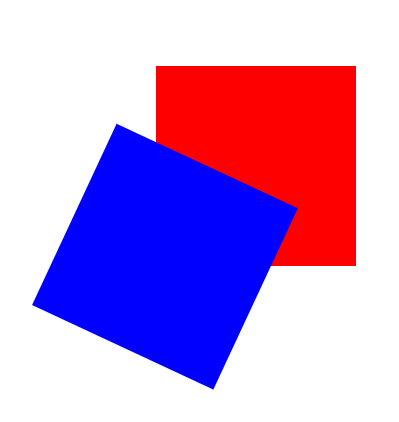
\includegraphics[width=7cm]{ss_html/canvas_rotate.png}
\end{figure}

El método \textbf{scale(x, y)} escala un gráfico, el parámetro \textit{x} indica la cantidad de veces que el gráfico será escalado en la dirección x, mientras que el parámetro \textit{y} indica la cantidad de veces que el gráfico será escalado en la dirección y. La \textit{Figura \ref{fig: 30}} muestra el resultado de un ejemplo de esta función:
\begin{lstlisting}
    <canvas id="canvas1" width="900" height="900"></canvas> 
            
    <script>
        var c=document.getElementById("canvas1");
        var ctx=c.getContext("2d");
        ctx.font="bold 22px Tahoma";
        ctx.textAlign="start";
        // Aspecto del texto en una ubicación.
        ctx.fillText("start", 10, 30);
        
        ctx.scale(1.5, 4);  // Escala el texto 1.5 veces en el eje X y 4 veces en el eje Y.

        // Mantiene el texto, pero lo ubica en otro sitio.
        ctx.fillText("start", 10, 60);
    </script>
\end{lstlisting}
\begin{figure}[H]
    \centering
    \caption{Escalando un gráfico con Canvas}
    \label{fig: 30}
    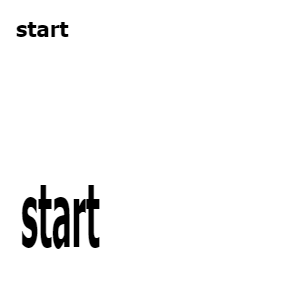
\includegraphics[width=5cm]{ss_html/canvas_scale.png}
\end{figure}

\textit{Nota}: si escala una figura, las futuras figuras estarán escaladas también.


\subsubsection{SVG vs Canvas}

La \textit{Tabla \ref{tab: 1}} compara las características de ambos métodos para dibujar figuras en documentos HTML:
\begin{table}[H]
    \begin{center}
        \caption{Comparación entre Canvas y SVG}
        \label{tab: 1}
        \begin{tabular}{m{7cm} m{7cm}}
            \hline
            \textbf{Canvas} & \textbf{SVG} \\
            \hline
            \begin{enumerate}
                \item Las figuras se dibujan por programación.
                \item El dibujo es por medio de píxeles.
                \item No maneja animaciones.
                \item Excelente rendimiento para figuras dibujadas con píxeles.
                \item Dependiente de la resolución.
                \item Sin manejadores de eventos.
                \item Se pueden guardar en formatos .png o .jpg.
                \item Muy adecuado para juegos con gráficos intensivos.
            \end{enumerate}
            &
            \begin{enumerate}
                \item Forman parte del DOM del sitio web.
                \item El dibujo es por medio de vectores.
                \item Maneja animaciones.
                \item Basado en XML estándar.
                \item Independiente de la resolución.
                \item Con manejadores de eventos.
                \item No muy adecuado para juegos.
                \item Muy adecuado para aplicaciones con grandes áreas de renderizado (por ejemplo, Google Maps).
            \end{enumerate}
            \\
            \hline
        \end{tabular}
    \end{center}
\end{table}

Podemos utilizar svg y canvas en un mismo sitio o página, pero no podemos dibujar figuras canvas dentro de un svg ni viceversa.


\subsection{Formularios HTML5}

La \textit{Tabla \ref{tab: 2}} contiene las etiquetas y atributos incorporados a esta versión de HTML, junto con ejemplos:
\begin{table}[H]
    \begin{center}
        \caption{Atributos y etiquetas nuevas de formularios en HTML5}
        \label{tab: 2}
        \begin{tabular}{m{2.5cm} m{7cm} m{5cm}}
            \hline
            \parbox{2.5cm}{\textbf{Atributo \\ Etiqueta}} & \textbf{Definición} & \textbf{Ejemplo} \\
            \hline
            autofocus       & Atributo que da el foco a un control cuando el sitio o página carga                                                           & \parbox{5cm}{$<$input type="text" \\ autofocus /$>$} \\
            required        & Atributo que vuelve a un control necesario para enviar el formulario                                                          & \parbox{5cm}{$<$input type="text" \\ required /$>$} \\
            autocomplete    & Atributo que permite que un control o formulario pueda ser llenado con valores que el usuario ha ingresado previamente        & \parbox{5cm}{$<$input type="text" \\ autocomplete="off" /$>$} \\
            list            & Atributo que puede convertir una caja de texto regular en un menú desplegable (con la posibilidad de escribir todavía)        & \parbox{5cm}{$<$input type="text" \\ id="cajita" \\ list="colores" /$>$} \\
            search          & Crea una caja de búsqueda                                                                                       & \parbox{5cm}{$<$input type="search" \\ id="buscador" \\ name="buscaitem" /$>$} \\
            datalist        & Control complemento para \textbf{search} que define una lista de pre-valores para la caja de búsqueda. El ID de la etiqueta \textit{datalist} debe ser igual al valor del atributo \textit{list} de un control para que las opciones del primero aparezcan en el segundo                                     & \parbox{5cm}{$<$datalist id="buscador"$>$ \\ $<$/datalist$>$} \\
            options         & Sub-control complemento para \textbf{select} o \textbf{datalist} que define una lista de opciones para el menú desplegable    & $<$option value="1"$>$ \\
            email           & Crea una caja para un correo                                                                                          & \parbox{5cm}{$<$input type="email" \\ placeholder= \\ "example@gmail.com" /$>$} \\
            url             & Crea una caja para una URL                                                                                            & \parbox{5cm}{$<$input type="url" \\ placeholder= \\ "google.com" /$>$} \\
            tel             & Crea una caja para un número de teléfono                                                                               & \parbox{5cm}{$<$input type="tel" \\ placeholder="123 456 \\ 7890" /$>$} \\
            \hline
        \end{tabular}
    \end{center}
\end{table}

Algunos otras \textbf{etiquetas} y \textit{atributos} que no fueron detallados son:
\begin{itemize}
    \item \textbf{color}.
    \item \textbf{date}.
    \item \textbf{datetime}.
    \item \textbf{datetime-local}.
    \item \textbf{month}.
    \item \textbf{number}.
    \item \textbf{range}.
    \item \textbf{time}.
    \item \textit{formaction}.
    \item \textit{formenctype}.
    \item \textit{formmethod}.
    \item \textit{formnovalidate}.
    \item \textit{formtarget}.
    \item \textit{height \& width}.
    \item \textit{list}.
    \item \textit{min \& max}.
    \item \textit{multiple}.
    \item \textit{patter (regexp)}.
    \item \textit{step}.
\end{itemize}


% Fin del documento.
\end{document}